\chapter{Método Empírico}

Esquematicamente, o método empírico pode ser descrito por cinco fases:
\begin{enumerate}
\item {\em Observação:} medições sobre algum aspecto do mundo
\item {\em Hipótese:} concepção de um modelo consistente com as observações
\item {\em Predição:} eventos são previstos de acordo com o modelo
\item {\em Verificação:} as predições são testadas fazendo-se novas observações
\item {\em Validação:} o processo se repete ajustando o modelo até que ele concorde com as observações
\end{enumerate}

Dois pontos centrais sobre o método empírico é que as verificações devem ser {\em reprodutíveis} e as hipóteses {\em falseáveis}.
Uma hipóstese que não pode ser falseada por observações (empíricamente) não é científica e a o processo de verificação deve poder ser feito por outros cientístas independentes.

O aspecto do mundo que pretendemos investigar nesta disciplina é o tempo de processamento de um algoritmo.
Lembre-se, porém, que um algoritmo é uma ideia que precede o advento dos computadores.
O algoritmo de Euclídes, por exemplo, data de 300 a.C., ou seja, séculos antes dos primeiros computadores começarem a ser construídos nos anos 40.
Embora o algoritmo seja um conceito matemático, uma série de pesquisadores tiveram a ideia de investigá-los de maneira empírica no final dos anos 60.
A série de livros The Art of Programing, de Donald Knuth, é um marco dessa abordagem dos estudos de algoritmos \cite{knuth97}.

Em nosso recorte, observaremos o tempo de processamento da execução de um programa para diferentes entradas.
Considere, por exemplo, o algoritmo para o problema da Busca apresentado no capítulo anterior:

\begin{codebox}
\Procname{$\proc{BuscaSequencial}(A, b)$}
\li \For $i \gets 1$ até $n$
\li \Do \If $a_i = b$
\li     \Then \Return $i$
        \End
    \End
\li \Return $\bot$
\End
\end{codebox}

Vamos implementar esse algoritmo na linguagem C de maneira direita:

\begin{lstlisting}[language=C]
  // devolve a posicao de n no arranjo ou -1 se nao encontrar
  int buscasequencial(int* array, int n, int size){
    int i;
    for(i = 0; i < size; i++)
      if(array[i] == n)
        return i;
    return -1;
  }      
\end{lstlisting}

Realizamos observações usando uma máquina específica (um notebook Dell com processador intel core i7 de $8^a$ geração de 1,9GHz) em um sistema operacional específico (Linux 5.11).
Medimos o tempo total de 300 buscas mal sucedidas em arranjos de tamanhos diferentes com valores inteiros positivos calculados aleatoriamente\footnote{Mais precisamente os valores seguem uma sequência pseudo-aleatória partindo de uma semente incial.}.
Os programas que calcula o tempo da busca e que gera as entradas estão disponíveis em \url{https://github.com/marciomr/IAA}.
Variamos o tamanho do arranjo entre um milhão e dez milhões.
Obtivemos o seguinte resultado para dez observações:

\begin{table}
  \label{tab:observacao}
  \begin{tabular}{|c|c|}
    \hline
    tamanho do arranjo em milhões & tempo de 300 buscas em segundos \\
    \hline 
    1                             & 0,99                            \\
    2                             & 2,08                            \\
    3                             & 3,12                            \\
    4                             & 3,99                            \\
    5                             & 5,05                            \\
    6                             & 5,94                            \\
    7                             & 7,03                            \\
    8                             & 7,92                            \\
    9                             & 8,93                            \\
    10                            & 9,85                            \\
    \hline
  \end{tabular}
\end{table}

As observações sugerem que para cada um milhão de valores no arranjo, o tempo de processamento aumenta mais ou menos um segundo.
Essa poderia ser nossa hipótese, mas podemos fazer algo um pouco mais sofisticado.
Vamos plotar os valores da tabela em um gráfico (Figura \ref{fig:observacao}).

\begin{figure}[htp]
  \label{fig:observacao}
  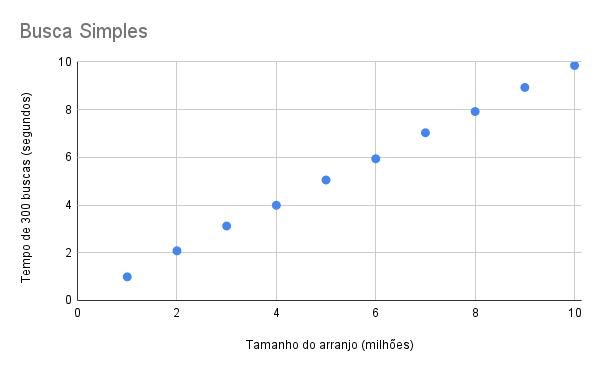
\includegraphics[width=0.9\textwidth]{imagens/grafico1.png}
  \caption{Tempo de processamento da busca simples.}
\end{figure}

Como os pontos estão mais ou menos alinhados e como é razoável supor que um arranjo sem nenhum elemento retornaria instantaneamente o resultado, faremos a hipótese de que o tempo de processamento segue uma função linear partindo do zero.
Ou seja, a seguinte função descreve o tempo de processamento da nossa implementação em nosso ambiente:

\begin{displaymath}
t(x) = a.x
\end{displaymath}

Podemos então usar uma regressão linear para estimar o valor de $a$ que minimize a distância desse reta para cada um dos pontos.
Obtemos então o valor $a = 0,997$.
Na Figura \ref{fig:hipotese} plotamos a função $t(x) = 0,997x$ no gráfico anterior.

\begin{figure}[htp]
  \label{fig:hipotese}
  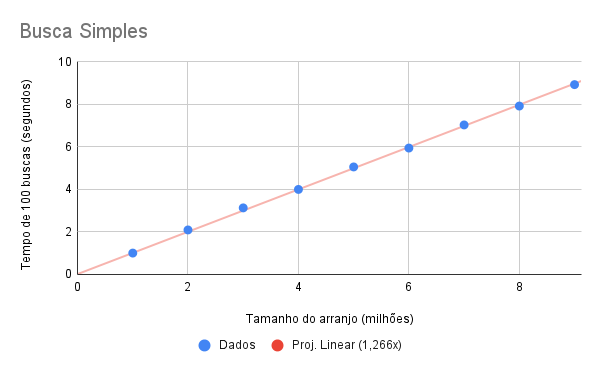
\includegraphics[width=0.9\textwidth]{imagens/grafico2.png}
  \caption{Gráfico ilustrando a hipótese de que o tempo de processamento da busca simples segue a função $t(x) = 0,997x$.}
\end{figure}

Podemos agora testar nossa hipótese de que o tempo de processamento da nossa implementação da busca sequencial para outros valores ainda não observados.
A segunda coluna da Tabela \ref{tab:verificacao} mostra os valores previstos pela hipótese para o tempo de processamento para entradas de tamanho 11 a 15 milhões.
Finalmente, podemos testar a hipótese.
Na última coluna da mesma tabela indicamos os valores observados para essas entradas:

\begin{table}
  \label{tab:verificacao}
  \begin{tabular}{|c|c|c|}
    \hline
    tamanho do arranjo em milhões & tempo previsto & tempo observado \\
    \hline 
    11                             & 10,97         & 10,87           \\
    12                             & 11,97         & 11,81           \\
    13                             & 12,97         & 12,78           \\
    14                             & 13,96         & 14,00           \\
    15                             & 14,96         & 14,74           \\
    \hline
  \end{tabular}
  \caption{Tempo de processamento previsto e observado para tamanhos maiores de arranjos.}
\end{table}

Os valores observados são notavelmente próximos aos previstos.
Ou seja, nossa hipótese foi verificada.
Poderíamos neste momento utilizar um teste estatístico para verificar nossa hipótese, mas isso foge do escopo desta disciplina.
Por hora diremos apenas que os dados parecem verificar a hipótese.

